\documentclass{beamer}
\usetheme{Boadilla}

\beamertemplatenavigationsymbolsempty 

\usepackage{diagbox}
\usepackage{tikz}
\usepackage{pgfplots}

\title{Selecting the `i'th largest of `n' elements}
\subtitle{with the fewest possible comparisons.}
\author{Die Bildungselite}
% \institute{FMI - University of Stuttgart}
\date{\today}


\begin{document}
\begin{frame}
    \titlepage
\end{frame}

\section{Outline}

\begin{frame}
    \frametitle{\insertsection}
    \begin{enumerate}[1.]
        \item Introduction
        \item Fundamentals
        \item Forward Search
        \item Backward search
        \item Results
    \end{enumerate}
\end{frame}

\section{Introduction}
\begin{frame}
    \frametitle{\insertsection} 


    \textit{Selection:} Select the $i$-th smallest element in a list with $n$ elements.

    \vspace{5mm} 
    Previous works: 

    \vspace{5mm}
    \begin{tabular}{|p{5cm}|p{5cm}|}
        \hline
        Gasarch, Kelly, and Puth & Oksanen \\ 
        \hline
        \raggedright \begin{itemize}
            \item Introduced computer search to find optimal selection algorithms.
            \item ...
        \end{itemize} & 
        \raggedright \begin{itemize}
            \item Published a computer search algorithm improving the previously known lower bounds found
            by Gasarch et. al. 
        \end{itemize}
    \end{tabular}
\end{frame}

\section{Poset}

\begin{frame}
    \frametitle{\insertsection}

    $$ \Omega = \{ a,b,c,...\}, \quad |\Omega| = n $$
    $$P = (n,i,R), \quad R \subseteq \Omega^2$$

\end{frame}

\begin{frame}
    \frametitle{\insertsection}

    \centering
    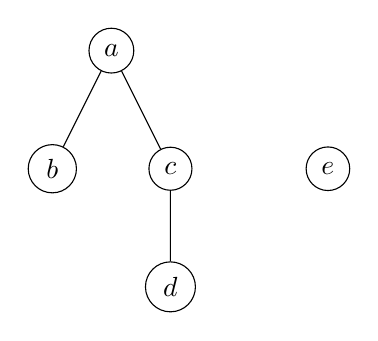
\begin{tikzpicture}

        \node[draw, circle] (a) {$a$}
        child {
                node[draw, circle] {$b$}
            }
        child {
                node[draw, circle] (c) {$c$}
                child {
                        node[draw, circle] {$d$}
                    }
            }
        ;

        \node[draw, circle, right of=c, node distance=2cm] {$e$};

    \end{tikzpicture}

    \begin{align*}
        a & > b \\
        a & > c \\
        c & > d
    \end{align*}

\end{frame}

\section{Compatible Solution}

\begin{frame}
    \frametitle{\insertsection}

    \centering
    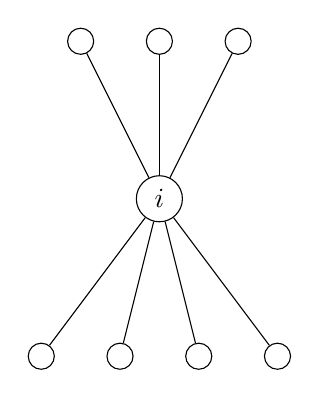
\begin{tikzpicture}
        
        \node[draw, circle] (l0) at (0, 0) {};
        \node[draw, circle] (l1) at (1, 0) {};
        \node[draw, circle] (l2) at (2, 0) {};
        \node[draw, circle] (l3) at (3, 0) {};
        
        \node[draw, circle] (I) at (1.5, 2) {$i$};

        \path[draw] (l0) to (I);
        \path[draw] (l1) to (I);
        \path[draw] (l2) to (I);
        \path[draw] (l3) to (I);

        \node[draw, circle] (u0) at (0.5, 4) {};
        \node[draw, circle] (u1) at (1.5, 4) {};
        \node[draw, circle] (u2) at (2.5, 4) {};

        \path[draw] (u0) to (I);
        \path[draw] (u1) to (I);
        \path[draw] (u2) to (I);

    \end{tikzpicture}

\end{frame}

\begin{frame}
    \frametitle{\insertsection}

    \centering
    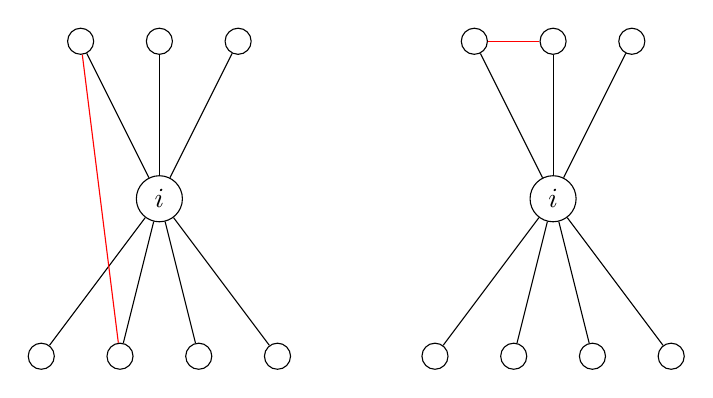
\begin{tikzpicture}
        
        \node[draw, circle] (fl0) at (0, 0) {};
        \node[draw, circle] (fl1) at (1, 0) {};
        \node[draw, circle] (fl2) at (2, 0) {};
        \node[draw, circle] (fl3) at (3, 0) {};
        
        \node[draw, circle] (fI) at (1.5, 2) {$i$};

        \path[draw] (fl0) to (fI);
        \path[draw] (fl1) to (fI);
        \path[draw] (fl2) to (fI);
        \path[draw] (fl3) to (fI);

        \node[draw, circle] (fu0) at (0.5, 4) {};
        \node[draw, circle] (fu1) at (1.5, 4) {};
        \node[draw, circle] (fu2) at (2.5, 4) {};

        \path[draw] (fu0) to (fI);
        \path[draw] (fu1) to (fI);
        \path[draw] (fu2) to (fI);

        \path[draw=red] (fu0) to (fl1);

        %second

        \node[draw, circle] (sl0) at (0 + 5, 0) {};
        \node[draw, circle] (sl1) at (1 + 5, 0) {};
        \node[draw, circle] (sl2) at (2 + 5, 0) {};
        \node[draw, circle] (sl3) at (3 + 5, 0) {};
        
        \node[draw, circle] (sI) at (1.5 + 5, 2) {$i$};

        \path[draw] (sl0) to (sI);
        \path[draw] (sl1) to (sI);
        \path[draw] (sl2) to (sI);
        \path[draw] (sl3) to (sI);

        \node[draw, circle] (su0) at (0.5 + 5, 4) {};
        \node[draw, circle] (su1) at (1.5 + 5, 4) {};
        \node[draw, circle] (su2) at (2.5 + 5, 4) {};

        \path[draw] (su0) to (sI);
        \path[draw] (su1) to (sI);
        \path[draw] (su2) to (sI);

        \path[draw=red] (su0) to (su1);

    \end{tikzpicture}

\end{frame}

\section{Forward Search}

\begin{frame}
    \frametitle{\insertsection}



\end{frame}

\begin{frame}
    \frametitle{\insertsection}

    \centering
    \begin{tikzpicture}
        [
            level 1/.style = {sibling distance = 4cm},
            level 2/.style = {sibling distance = 2.5cm},
        ]

        \node[] (root) {$(n,i,\emptyset)$}
        child {
                node[] {$\{a,b\}$}
                child {
                        node[] {$(n,i,\{(a,b)\})$}
                        child[sibling distance = 1cm] {
                                node[] {$\{c,d\}$}
                                child[sibling distance = 1cm] { node[] {$\cdots$}}
                                child[sibling distance = 1cm] { node[] {$\cdots$}}
                            }
                        child[sibling distance = 1cm] { node[] {$\cdots$}}
                    }
                child {
                        node[] {$(n,i,\{(b,a)\})$}
                        child[sibling distance = 1cm] {
                                node[] {$\{c,d\}$}
                                child[sibling distance = 1cm] { node[] {$\cdots$}}
                                child[sibling distance = 1cm] { node[] {$\cdots$}}
                            }
                        child[sibling distance = 1cm] { node[] {$\cdots$}}
                    }
            }
        child {
                node {$\{a,c\}$}
                child[sibling distance = 1cm] { node[] {$\cdots$}}
                child[sibling distance = 1cm] { node[] {$\cdots$}}
            }
        child {
                node[] {$\cdots$}
            }
        ;

    \end{tikzpicture}

\end{frame}

\subsection{Multithreading}

\begin{frame}
    \frametitle{\insertsubsection}



\end{frame}

\section{Backward Search}

\begin{frame}
    \frametitle{\insertsection}

    Backward search

\end{frame}

\begin{frame}
    \frametitle{\insertsection}

    \centering

    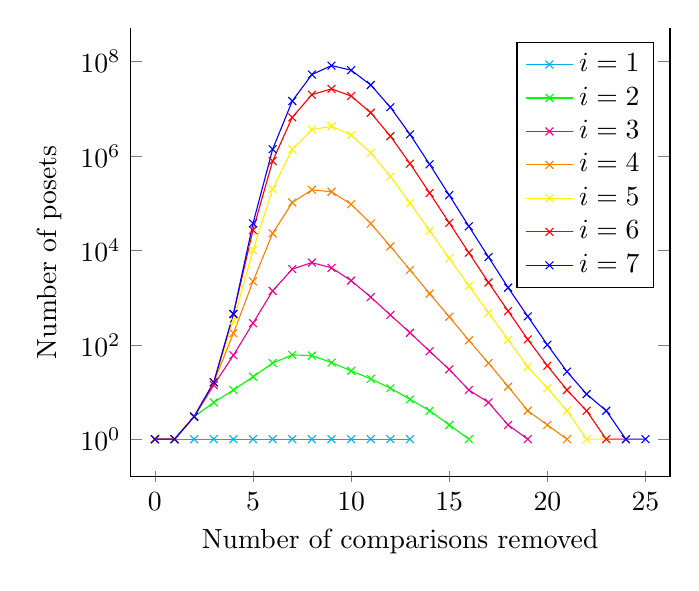
\begin{tikzpicture}
  \begin{axis}[
      ymode=log,
      axis x line = bottom,%x-Achse nur unten
      % x dir=reverse,
      enlarge x limits = .05,%x-Achse erweitern
      x axis line style = {-},%kein Pfeil
      % title = {\dots},
      ylabel={Number of posets},
      xlabel={Number of comparisons removed},
      % only marks,
      cycle list={{mark=x}},
      legend pos=north east,
    ]
    \addlegendentry{$i = 1$}
    \addplot+[cyan] table { %n=14,i=0
        x  y
        0  1
        1  1
        2  1
        3  1
        4  1
        5  1
        6  1
        7  1
        8  1
        9  1
        10 1
        11 1
        12 1
        13 1
      };
    \addlegendentry{$i = 2$}
    \addplot+[green] table { %n=14,i=1
        x y
        0  1
        1  1
        2  3
        3  6
        4  11
        5  21
        6  41
        7  61
        8  59
        9  42
        10 28
        11 19
        12 12
        13 7
        14 4
        15 2
        16 1
      };
    \addlegendentry{$i = 3$}
    \addplot+[magenta] table { %n=14,i=2
        x y
        0  1
        1  1
        2  3
        3  14
        4  60
        5  287
        6  1385
        7  4005
        8  5510
        9  4268
        10 2284
        11 1025
        12 428
        13 180
        14 73
        15 30
        16 11
        17 6
        18 2
        19 1
      };
    \addlegendentry{$i = 4$}
    \addplot+[orange] table { %n=14,i=3
        x y
        0  1
        1  1
        2  3
        3  16
        4  175
        5  2201
        6  22900
        7  103210
        8  191627
        9  174416
        10 94785
        11 37004
        12 12173
        13 3851
        14 1211
        15 392
        16 124
        17 41
        18 13
        19 4
        20 2
        21 1
      };
    \addlegendentry{$i = 5$}
    \addplot+[yellow] table { %n=14,i=4
        x y
        0  1
        1  1
        2  3
        3  16
        4  323
        5  10111
        6  200521
        7  1386176
        8  3607272
        9  4267576
        10 2763862
        11 1162696
        12 367875
        13 100552
        14 26024
        15 6745
        16 1781
        17 474
        18 127
        19 34
        20 12
        21 4
        22 1
        23 1
      };
    \addlegendentry{$i = 6$}
    \addplot+[red] table { %n=14,i=5
        x y
        0  1
        1  1
        2  3
        3  16
        4  446
        5  26921
        6  780123
        7  6588569
        8  19882832
        9  26416869
        10 18631911
        11 8243306
        12 2630332
        13 688904
        14 164372
        15 38334
        16 8918
        17 2084
        18 518
        19 130
        20 36
        21 11
        22 4
        23 1
        24 1
      };
    \addlegendentry{$i = 7$}
    \addplot+[blue] table { % n=14,i=6
        x y
        0  1
        1  1
        2  3
        3  16
        4  452
        5  37236
        6  1389385
        7  14591680
        8  53003482
        9  82198656
        10 65707713
        11 31909980
        12 10770689
        13 2864659
        14 665109
        15 147573
        16 32349
        17 7214
        18 1624
        19 400
        20 100
        21 27
        22 9
        23 4
        24 1
        25 1
      };
  \end{axis}
\end{tikzpicture}

\end{frame}

\section{Bidirectional Search}

\begin{frame}
    \frametitle{\insertsection}

    Bidirectional search

\end{frame}

\section{Results}

\begin{frame}
    \frametitle{\insertsection}

    \centering

    {\color{red} Rot: Rückwärtssuche},
    {\color{blue} Blau: Vorwärtssuche}

    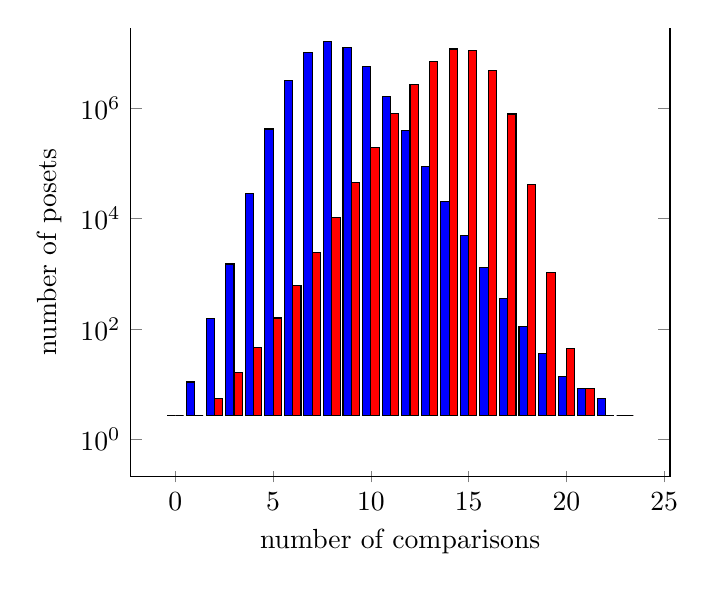
\begin{tikzpicture}
  \begin{axis}[
      ybar,
      ymode=log,
      axis x line = bottom,%x-Achse nur unten
      enlarge x limits = .1,%x-Achse erweitern
      x axis line style = {-},%kein Pfeil
      bar width=3pt,
      ylabel={number of posets},
      xlabel={number of comparisons},
      % legend cell align=left,
      % legend pos=outer north east,
      % legend style={at={(0.5,-0.2)},anchor=north}, % draw=none
    ]
    % \addlegendentry{forward search}
    \addplot[fill=blue,shift={(1pt, 0)}] table {
        x y
        0  1
        1  4
        2  57
        3  552
        4  10397
        5  154828
        6  1166640
        7  3770182
        8  5941732
        9  4726819
        10 2096404
        11 604582
        12 143058
        13 32460
        14 7450
        15 1823
        16 471
        17 132
        18 41
        19 13
        20 5
        21 3
        22 2
        23 1
      };
    % \addlegendentry{backward search}
    \addplot[fill=red,shift={(-1pt, 0)}] table {
        x y
        23 1
        22 1
        21 3
        20 16
        19 381
        18 15227
        17 290138
        16 1750707
        15 4058631
        14 4368185
        13 2592437
        12 1006071
        11 291970
        10 72346
        9  16728
        8  3898
        7  893
        6  227
        5  58
        4  17
        3  6
        2  2
        1  1
        0  1
      };
  \end{axis}
\end{tikzpicture}

Treff: 11

\end{frame}

\begin{frame}
    \frametitle{\insertsection}

    \begin{table}
        \centering
        \begin{tabular}{c|cccccccc}
            \backslashbox{$n$}{$i$} & 0  & 1  & 2  & 3  & 4  & 5  & 6  & 7  \\ \hline
            1                       & 0                                     \\
            2                       & 1                                     \\
            3                       & 2  & 3                                \\
            4                       & 3  & 4                                \\
            5                       & 4  & 6  & 6                           \\
            6                       & 5  & 7  & 8                           \\
            7                       & 6  & 8  & 10 & 10                     \\
            8                       & 7  & 9  & 11 & 12                     \\
            9                       & 8  & 11 & 12 & 14 & 14                \\
            10                      & 9  & 12 & 14 & 15 & 16                \\
            11                      & 10 & 13 & 15 & 17 & 18 & 18           \\
            12                      & 11 & 14 & 17 & 18 & 19 & 20           \\
            13                      & 12 & 15 & 18 & 20 & 21 & 22 & 23      \\
            14                      & 13 & 16 & 19 & 21 & 23 & 24 & 25      \\
            15                      & 14 & 17 & 20 & 23 & 24 & 26 & 26 & 27 \\
        \end{tabular}
    \end{table}

\end{frame}

\end{document}